\documentclass[12pt, a4paper]{article}
\usepackage[
  margin=1in
]{geometry}
\usepackage{graphicx}
\usepackage{minted}
\usepackage[T1, T2A]{fontenc}
\usepackage[utf8]{inputenc}
\usepackage[russian]{babel}

\graphicspath{ {./img/} }

\begin{document}
\begin{titlepage}
  \centering
  \textsc{Новосибирский государственный технический университет}\par
  \vspace{1mm}
  Кафедра теоретической и прикладной информатики\par
  \vspace{4cm}
  \textsc{Расчетно-графическая работа}\par
  {\huge\bfseries Алгоритм сжатия данных\par}
  \vspace{1cm}
  {\scriptsize ФПМИ, ПМ-24\par}
  \vspace{1mm}
  {\itshape\large Параскун И., Герасименко В.\par}
  \vfill
  {\small преподаватель\par}
  \vspace{1mm}
  \textsc{Сивак Мария Алексеевна}
  \vfill
  \large{Новосибирск, 2024}
\end{titlepage}

\tableofcontents

\newpage

\section{Введение}
Данная расчетно-графическая работа представляет собой комплекс проведенных
теоретических и прикладных исследований.
\subsection{Алгоритм Хаффмана}
Первой частью работы стало изучение алгоритма Хаффмана в качестве
алгоритма сжатия данных, выявление его преимуществ и недостатков, а также
определение оптимальных условий для его применения.
\subsection{Практическая реализация}
Вторая часть состояла в практической реализации изученного алгоритма.
Задача заключалась в том, чтобы предоставить компактное решение реальной
проблемы - сжатие данных.

\section{Теоретическая часть}
Алгоритм Хаффмана - алгоритм оптимального префиксного кодирования алфавита.
Основная используемая структура данных - дерево Хаффмана.
\subsection{Дерево Хаффмана}
Дерево Хаффмана представляет собой бинарное дерево со свойствами кучи, листья -
кодируемые символы.
Существует два варианта исполнения - статический и динамический.
\subsubsection{Статическое дерево Хаффмана}
Статическое дерево Хаффмана представляет собой дерево со свойствами
бинарной кучи. В дереве закодирован предопределенный набор символов
(например, английский алфавит) на основе исследований о средней
частоте их использования.
\vspace{3mm}
\begin{center}
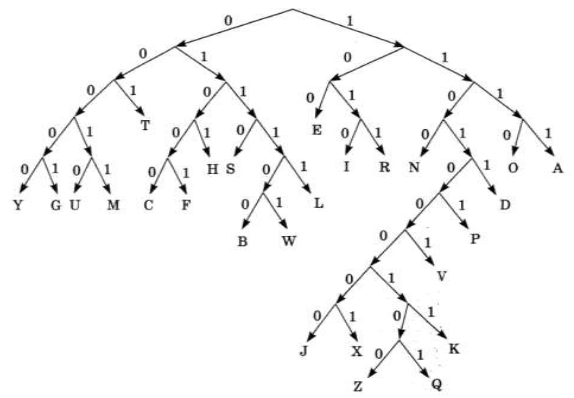
\includegraphics[scale=0.5]{tree.png}
\end{center}
\subsubsection{Динамическое дерево Хаффмана}
Динамическое дерево Хаффмана строится по кодируемому файлу во время
первого обхода. Коды получаются меньше, чем в статической реализации, однако
появляется необходимость в записи дополнительной информации о частоте символов.

\section{Описание программы}
Программа состоит из вспомогательных модулей, подпрограмм
кодирования и декодирования.
\subsection{Вспомогательные модули}
\subsubsection{Очередь по приоритетам}
Очередь по приоритетам необходима для построения дерева Хаффмана.
Выбранная реализация - бинарная куча, первый элемент которой - узел дерева
с минимальной частотой.\\
Асимтотические оценки:
\begin{itemize}
  \item Вставка - $\mathcal{O}(\log{n})$
  \item Извлечение - $\mathcal{O}(\log{n})$ 
  \item Изменение - $\mathcal{O}(\log{n})$
\end{itemize}
\subsubsection{Дерево Хаффмана}
Дерево Хаффмана (\ref{listing:1}) реализовано по принципу связного списка. Каждое звено,
помимо основной информации, хранит свой индекс в очереди,
ссылку на левого потомка и ссылку на правого потомка.\\
Основной модуль - подпрограмма построения дерева (\ref{listing:2}).
\subsection{Структура данных в памяти}
Результат выполения программы сохраняется в память следующим образом:
\begin{center}
  
\includegraphics[scale=0.45]{mem.png}
\end{center}
Здесь, единичный квадратик - 1 байт, $lbs$ - число бит в последнем байте
кодового пространства, $n$ - число уникальных символов. Для каждого
уникального символа ($s_n$) хранится соответсвующая ему частота ($f_n$).
\subsection{Подпрограмма кодирования}
В общем виде алгоритм кодирования (\ref{listing:3}) выглядит следующим образом:
\begin{enumerate}
  \item Чтение входного файла, составление очереди.
  \item Построение дерева Хаффмана.
  \item Повторное чтение входного файла, запись кодового пространства в
  результирующий файл.
  \item Запись мета информации в результирующий файл.
\end{enumerate}
Алгоритм построения дерева Хаффмана модифицирует данную ему очередь. В
связи с этим, очередь, после построения, должна быть скопирована для
дальнейшего занесения в мета информацию.
\subsection{Подпрограмма декодирования}
Алгоритм декодирования (\ref{listing:4}):
\begin{enumerate}
  \item Чтение мета информации из входного файла.
  \item Построение дерева Хаффмана.
  \item Чтение кодового пространства из входного файла, обход дерева и
  запись результата в файл.
\end{enumerate}
Пары символ-частота сохраняются в мета блоке в том порядке, в котором они
находились во внутреннем массиве очереди, а не по приоритетам. Это позволяет
сразу составить требуемую для алгоритма декодирования очередь, без
необходимости восстановления свойств бинарной кучи.

\section{Результаты тестирования}
\subsection{Корректность представления}
Для проверки соотвествия представления заявленному, приведем простой
тестовый файл и результат работы алгоритма сжатия:\\
\begin{minted}{text}
Входной текст (in.txt):
ABC

Результат (in.txt.huff):
00000000  08 04 41 01 00 00 00 00  00 00 00 42 01 00 00 00  |..A........B....|
00000010  00 00 00 00 43 01 00 00  00 00 00 00 00 0a 01 00  |....C...........|
00000020  00 00 00 00 00 00 39                              |......9|
00000027
\end{minted}
\textit{*четвертый символ - символ переноса строки. Он имеет ASCII код 0a.}

\subsection{Кодирование ASCII символов}
\begin{minted}{text}
Входной текст (build.gradle):
plugins {
    id 'cpp-application'
}

application {
    binaries.configureEach {
        def compileTask = compileTask.get()

        compileTask.source.from fileTree(dir: "src/main/c", include: "**/*.c")
        compileTask.compilerArgs = ["-x", "c", "-std=c11", "-g3"]

        def linkTask = linkTask.get().linkerArgs = ["-nodefaultlibs", "-lc"]
    }
}

Результат:
357* build.gradle
592* build.gradle.huff
\end{minted}
\textit{*размер файла в байтах}

\subsection{Кодирование не-ASCII символов}
\begin{minted}{text}
Входной текст (in.txt):
ABC

Первый круг:
00000000  08 04 41 01 00 00 00 00  00 00 00 42 01 00 00 00  |..A........B....|
00000010  00 00 00 00 43 01 00 00  00 00 00 00 00 0a 01 00  |....C...........|
00000020  00 00 00 00 00 00 39                              |......9|
00000027

Второй круг:
00000000  06 09 08 01 00 00 00 00  00 00 00 04 01 00 00 00  |................|
00000010  00 00 00 00 41 01 00 00  00 00 00 00 00 0a 01 00  |....A...........|
00000020  00 00 00 00 00 00 00 1c  00 00 00 00 00 00 00 42  |...............B|
00000030  01 00 00 00 00 00 00 00  43 01 00 00 00 00 00 00  |........C.......|
00000040  00 01 04 00 00 00 00 00  00 00 39 01 00 00 00 00  |..........9.....|
00000050  00 00 00 63 96 7f 43 fa  8f ef 3f b4              |...c..C...?.|
0000005c
\end{minted}

\subsection{Кодирование специализированных файлов}
Под специализированностью понимается низкая уникальность и высокая частотность.

\begin{minted}{text}
Входной текст (in.txt):
AAAAAAAAAAAAAAAAAAAAAAAAAAAAAAAAAAAAAAAAAAAAAAAAAAAAAAAAAAAAAA
BBBBBBBBBBBBBBBBBBBBBBBBBBBBBBBBBBBBBBBBBBBBBBBBBBBBBBBBBBBBB
CCCCCCCCCCCCCCCCCCCCCCCCCCCCCCCCCCCCCCCCCCCCCCCCCCCCCCCCCCCC
DDDDDDDDDDDDDDDDDDDDDDDDDDDDDDDDDDDDDDDDDDDDDDDDDDDDDDDDDDD
EEEEEEEEEEEEEEEEEEEEEEEEEEEEEEEEEEEEEEEEEEEEEEEEEEEEEEEEEE
FFFFFFFFFFFFFFFFFFFFFFFFFFFFFFFFFFFFFFFFFFFFFFFFFFFFFFFFF
GGGGGGGGGGGGGGGGGGGGGGGGGGGGGGGGGGGGGGGGGGGGGGGGGGGGGGGG

Результат (in.txt.huff):
00000000  04 08 0a 07 00 00 00 00  00 00 00 47 38 00 00 00  |...........G8...|
00000010  00 00 00 00 46 39 00 00  00 00 00 00 00 44 3b 00  |....F9.......D;.|
00000020  00 00 00 00 00 00 43 3c  00 00 00 00 00 00 00 42  |......C<.......B|
00000030  3d 00 00 00 00 00 00 00  45 3a 00 00 00 00 00 00  |=.......E:......|
00000040  00 41 3e 00 00 00 00 00  00 00 ff ff ff ff ff ff  |.A>.............|
00000050  ff ff ff ff ff ff ff ff  ff ff ff ff ff ff ff ff  |................|
00000060  ff c6 db 6d b6 db 6d b6  db 6d b6 db 6d b6 db 6d  |...m..m..m..m..m|
00000070  b6 db 6d b6 db 6d b6 db  61 6d b6 db 6d b6 db 6d  |..m..m..am..m..m|
00000080  b6 db 6d b6 db 6d b6 db  6d b6 db 6d b6 db 6d a2  |..m..m..m..m..m.|
00000090  49 24 92 49 24 92 49 24  92 49 24 92 49 24 92 49  |I$.I$.I$.I$.I$.I|
000000a0  24 92 49 24 92 48 1b 6d  b6 db 6d b6 db 6d b6 db  |$.I$.H.m..m..m..|
000000b0  6d b6 db 6d b6 db 6d b6  db 6d b6 db 09 24 92 49  |m..m..m..m...$.I|
000000c0  24 92 49 24 92 49 24 92  49 24 92 49 24 92 49 24  |$.I$.I$.I$.I$.I$|
000000d0  92 48 12 49 24 92 49 24  92 49 24 92 49 24 92 49  |.H.I$.I$.I$.I$.I|
000000e0  24 92 49 24 92 49 24 80                           |$.I$.I$.|
000000e8

420 in.txt
232 in.txt.huff
\end{minted}

\section{Заключение}
\subsection{Условия применения алгоритма}
Результаты тестирования показывают, что \textbf{динамическая} реализация алгоритма
на произвольном наборе ASCII символов менее эффективна, чем на специализированных наборах.
Таким образом, чистое применение алгоритма Хаффмана целесообразно только для решения
узконаправленных задач. В остальных же случаях, рекомендуется использовать его в комбинации
с другими алгоритмами (что и делается в большинстве распространенных
алгоритмов сжатия).
\subsection{Недостатки реализации}
\begin{enumerate}
  \item Размер блока с частотой статический, что увеличивает пространство мета информации
  на диске.
\end{enumerate}

\begin{listing}
\inputminted{c}{src/htree.h}
\caption{Интерфейс дерева Хаффмана}
\label{listing:1}
\end{listing}

\begin{listing}
\inputminted[firstline=7, lastline=33]{c}{src/htree.c}
\caption{Подпрограмма построения дерева Хаффмана}
\label{listing:2}
\end{listing}

\begin{listing}
\inputminted[firstline=23, lastline=66]{c}{src/huff.c}
\caption{Подпрограмма кодирования}
\label{listing:3}
\end{listing}

\begin{listing}
\inputminted[firstline=74, lastline=107]{c}{src/huff.c}
\caption{Подпрограмма декодирования}
\label{listing:4}
\end{listing}
\end{document}
